\documentclass[a4paper,conference]{IEEEtran}
\IEEEoverridecommandlockouts

\usepackage{cite}
\usepackage{amsmath,amssymb,amsfonts}
\usepackage{graphicx}
\usepackage{booktabs}
\usepackage{array}
\usepackage{textcomp}
\usepackage{xcolor}
\usepackage{tikz}
\usetikzlibrary{arrows.meta,positioning}
\usepackage{pgfplots}
\pgfplotsset{compat=1.17}

\newcommand{\HIGH}{\textsc{high}}
\newcommand{\MED}{\textsc{medium}}
\newcommand{\LOW}{\textsc{low}}

\begin{document}

\title{Risk-Adaptive Late-Binding Decryption for\\ Field-Level Exposure Control in Backend Systems}

\author{\IEEEauthorblockN{Anonymous Author(s)}
\IEEEauthorblockA{\textit{Affiliation withheld for double-blind review}}}

\maketitle

\begin{abstract}
Field-level application encryption keeps sensitive columns unreadable in storage, but a
conventional backend gives that protection away at the worst possible moment: the
object-relational mapper (ORM) decrypts every protected column while it hydrates an entity,
before any code has examined who is asking or how that principal is behaving. A stolen token,
an enumeration script, or a misused staff account therefore receives plaintext as soon as it
clears a static role check. This paper presents a backend framework that reorders those two
steps. Protected columns survive retrieval as ciphertext, six server-derived signals are
encoded into an eight-element vector and classified as \LOW{}, \MED{} or \HIGH{} risk by a
75-tree random forest, and the predicted tier selects full decryption, partial decryption with
masking, or refusal before any decryption call is made. The classifier is trained on a
reproducible synthetic corpus of 10{,}000 rule-labelled access events. On a quarantined
1{,}500-event partition it reaches 0.9780 accuracy, 0.9777 weighted F1 and 0.9407 macro F1,
serving 99.14\% of legitimate requests in full while refusing 92.81\% of the simulated abusive
ones; repeating the whole procedure on five independently generated corpora gives
$0.9797 \pm 0.0033$ weighted F1. The trained forest is transpiled to plain JavaScript and runs
inside the Node.js process: it reproduces the Python predictions on all 1{,}500 test rows
(largest probability deviation $1.3\times10^{-15}$) with a median warm latency of 23.6~$\mu$s.
End-to-end runs on the integrated backend confirm the intended behaviour, with 7, 2 and 0
field decryptions on the three paths. Results are reported as a synthetic proof of concept, not
as evidence of real-world attack detection.
\end{abstract}

\begin{IEEEkeywords}
data-in-use protection, application-level encryption, adaptive access control, random forest,
model transpilation, backend security
\end{IEEEkeywords}

\section{Introduction}

Most production backends protect data reasonably well in two of its three states. Disks and
backups are covered by transparent database encryption, traffic is covered by TLS, and
application-level encryption (ALE) narrows the trust boundary further by encrypting individual
sensitive fields before they ever reach the database. What remains unguarded is the moment the
data becomes usable. In a typical ORM setup, an encrypted column is declared with a value
transformer whose load-path function decrypts automatically. Any query that touches the row
therefore materialises plaintext in process memory as a side effect, long before the service
layer has decided whether this particular request deserves it.

The consequence is an ordering problem rather than a cryptographic one. The cipher does its
job; the decision to invoke it is simply never examined. Attacks that hold valid credentials
exploit exactly this gap. An insecure direct object reference (IDOR) attempt reads another
customer's row, a scraping script walks an endpoint at forty requests per minute, and an account
that has just been taken over after a burst of failed logins behaves like any other authenticated
session. Static role-based access control (RBAC) answers only whether the caller may invoke the
endpoint, and it answers once. It has no vocabulary for ``this caller may proceed, but should
not see the account number this time.''

This paper takes the position that decryption itself should be the enforcement point. We keep
authentication and static authorisation as mandatory controls, then insert one additional
decision immediately before the cryptographic boundary. Protected fields are retrieved as
ciphertext, a small feature vector is assembled from evidence the client cannot forge, a
classifier assigns a risk tier, and that tier decides how much of the record is decrypted --- all
of it, two display fields with the primary identifier masked, or nothing at all.

The contributions are as follows.
\begin{enumerate}
\item A ciphertext-preserving ORM design in which entity hydration performs no decryption, so
      that decryption becomes an explicit call that exactly one component is allowed to make.
\item A graduated three-tier exposure policy whose middle tier keeps a workflow usable while
      withholding the high-value identifiers, including masking of the account number with zero
      decryption operations.
\item An in-process risk model obtained by transpiling a trained random forest into plain
      JavaScript, removing the inference service, the network hop and the language boundary from
      the request path.
\item An evaluation covering held-out classification quality, repetition over five independently
      generated corpora, exact Python--JavaScript agreement on the full test partition, latency
      percentiles, and end-to-end field-level exposure counts on the integrated backend.
\end{enumerate}

\section{Related Work}

Authenticated encryption with AES-GCM is the standard building block for field-level protection
and provides confidentiality and integrity under a unique nonce per operation~\cite{gcm}.
Storage- and database-level encryption protect files, media and backups~\cite{tde,atrest}, and
surveys of database security treat encryption and access control as complementary
layers~\cite{dbsurvey}. All of these mechanisms act before decryption. None of them constrains
how much plaintext an already-running, already-authorised code path should produce.

RBAC~\cite{rbac} and ABAC~\cite{abac,abacopen} supply the deterministic authorisation structure
that backends actually deploy. Zero Trust guidance~\cite{zta,zt5} argues that authentication
should not be treated as a one-time grant and that verification should continue per request, and
risk-adaptive access control adds a quantified risk term to the authorisation
decision~\cite{riskabac}. Machine learning has been applied to that decision in several
forms: permission-decision engines trained on historical grants~\cite{mlengine}, hybrid access
control for industrial networks~\cite{scada}, and risk-adaptive ABAC for IoT
deployments~\cite{riskabac}. A recent systematic mapping of context-aware and ML-assisted access
control~\cite{survey} confirms the general pattern: the learned score feeds an admission
decision, and the enforcement point is the policy engine.

Two properties of that literature motivate the present work. First, the decision remains
admission-shaped. Once a request is admitted, the response is produced in full, so a system that
is unsure about a request can only choose between serving everything and blocking everything.
Second, the risk model normally sits outside the request path, in a separate service or an
offline analytics pipeline, which makes per-read scoring expensive and pushes deployments toward
after-the-fact alerting. What we did not find in the reviewed work is the combination of four
elements in one backend: retrieval that preserves ciphertext, a per-request behavioural score
computed from server-controlled evidence, a graduated policy that can partially decrypt, and
inference cheap enough to run on every sensitive read.

\section{Proposed Framework}

\subsection{Threat model}

We assume the attacker holds valid credentials and passes both authentication and static
authorisation. This covers stolen or replayed tokens, accounts compromised through credential
stuffing, IDOR-style enumeration by a legitimate customer account, automated scraping through a
valid session, and misuse by staff whose role legitimately permits cross-record reads. The
attacker is assumed to control only request content and timing; the JWT signature, the server
clock and the server-side audit tables are outside their reach. Attacks against the database
files, the key material, or the transport channel are out of scope --- those are the province of
storage encryption, key management and TLS respectively, and the framework assumes they remain
in place beneath it.

\subsection{Late-binding application-level encryption}

The pivot of the design is a two-line change with architectural consequences. In the standard
value transformer the save path encrypts and the load path decrypts. We keep the save path
unchanged --- fields are sealed with AES-256-GCM under a fresh 96-bit IV into a versioned
envelope \texttt{version:iv:tag:ciphertext} --- and make the load path return the stored string
untouched:

\begin{center}
\small
\texttt{from(v) \{ return v; \} \quad // ciphertext survives hydration}
\end{center}

A repository query now yields an entity whose sensitive properties are ciphertext strings.
Retrieval performs no application-level decryption at all, decryption becomes an explicit call
that only the adaptive layer is permitted to make, and the ordering inverts from ``decrypt, then
perhaps authorise'' to ``assess, then perhaps decrypt.'' One schema detail supports the middle
tier: the last four digits of the account number are stored in a separate plaintext column, so a
masked account number can be rendered without touching its ciphertext.

\subsection{Request context}

Each protected read is described by six business features, listed in Table~\ref{tab:features}.
All six come from sources the caller cannot influence except by genuinely behaving differently:
the verified token claim, a sensitivity tier declared statically by the domain module, the server
clock, the owner column of the row that was just fetched, and two indexed range queries over
audit tables. Ownership is compared against the fetched row rather than against any
client-supplied parameter. The velocity window is 60 seconds and the request being scored is
included in its own count, since its audit row is inserted before scoring. The failure window is
deliberately long at 24 hours: a short window would reset to zero at precisely the moment a
credential-stuffing attacker finally succeeds and starts reading data.

\begin{table}[t]
\caption{Runtime features and their server-side sources.}
\label{tab:features}
\centering
\footnotesize
\begin{tabular}{@{}lll@{}}
\toprule
Feature & Encoding & Source \\
\midrule
Role & 3 one-hot & Verified token claim \\
Sensitivity tier & $\{0,1,2\}$ & Declared by domain module \\
Office hours & $\{0,1\}$ & Server clock, Mon--Fri 09--17 \\
Owner match & $\{0,1\}$ & Token subject vs.\ row owner \\
60-s request count & integer & Access-request log \\
24-h failed logins & integer & Authentication log \\
\bottomrule
\end{tabular}
\end{table}

Because a fitted encoder cannot be exported to JavaScript, the six features are expanded by
stateless hand-written mappings into an invariant eight-element vector
\begin{equation}
\mathbf{x}=[r_c,\; r_m,\; r_a,\; s,\; h,\; o,\; v,\; f]^{\top}\in\mathbb{R}^{8},
\end{equation}
where $r_c,r_m,r_a$ are the one-hot role indicators, $s\in\{0,1,2\}$ the sensitivity tier,
$h$ the office-hours flag, $o$ the ownership match, $v$ the 60-second request count and $f$ the
24-hour failure count. The same index assignment is used by the Python training code and by the
TypeScript runtime; any reordering would silently corrupt every prediction, which is why it is
checked by the parity test of Section~\ref{sec:parity}.

\subsection{Risk model and graduated policy}

The classifier is a random forest~\cite{rf} of $T=75$ trees with maximum depth 12 and balanced
class weights. For class $c$ the forest averages the per-tree distributions,
\begin{equation}
\hat p(c\mid\mathbf{x})=\frac{1}{T}\sum_{t=1}^{T}p_t(c\mid\mathbf{x}),
\qquad
\hat c=\arg\max_{c}\;\hat p(c\mid\mathbf{x}),
\end{equation}
and a deterministic policy $\pi$ maps the predicted tier to a cryptographic action:
$\pi(\LOW)=\textsc{full}$, $\pi(\MED)=\textsc{partial}$, $\pi(\HIGH)=\textsc{deny}$. The
architectural invariant the implementation must satisfy is
\begin{equation}
N_{\text{decrypt}}(q)=0 \quad\text{whenever}\quad \pi(\hat c)=\textsc{deny},
\label{eq:invariant}
\end{equation}
that is, a refusal is raised before the first decryption call, so a correct \HIGH{}
classification prevents exposure rather than reporting it afterwards.

We chose a forest rather than a linear model because the security semantics are conjunctions
over several attributes at once, and rather than a neural model because the artifact has to
transpile to dependency-free arithmetic and stay auditable. Depth 12 was selected on the
validation partition; deeper forests gained nothing measurable and inflated the generated code.
Figure~\ref{fig:pipeline} shows how the pieces fit together at runtime.

\begin{figure}[t]
\centering
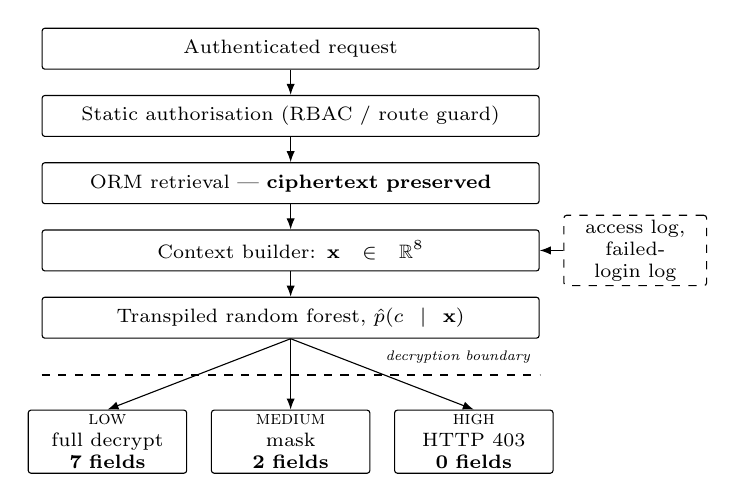
\begin{tikzpicture}[
  font=\scriptsize,
  node distance=3.2mm,
  box/.style={draw, rounded corners=1pt, align=center, inner sep=1.6pt,
              text width=62mm, minimum height=5.2mm},
  small/.style={draw, rounded corners=1pt, align=center, inner sep=1.6pt,
              text width=19mm, minimum height=8mm},
  side/.style={draw, dashed, rounded corners=1pt, align=center, inner sep=1.6pt,
              text width=17mm, minimum height=5mm},
  ar/.style={-{Latex[length=1.4mm]}}
]
\node[box] (req) {Authenticated request};
\node[box, below=of req] (auth) {Static authorisation (RBAC / route guard)};
\node[box, below=of auth] (orm) {ORM retrieval --- \textbf{ciphertext preserved}};
\node[box, below=of orm] (ctx) {Context builder: $\mathbf{x}\in\mathbb{R}^{8}$};
\node[box, below=of ctx] (rf) {Transpiled random forest, $\hat p(c\mid\mathbf{x})$};

\draw[ar] (req) -- (auth);
\draw[ar] (auth) -- (orm);
\draw[ar] (orm) -- (ctx);
\draw[ar] (ctx) -- (rf);

\node[small, below=9mm of rf] (med) {\MED\\ mask\\ \textbf{2 fields}};
\node[small, left=3mm of med] (low) {\LOW\\ full decrypt\\ \textbf{7 fields}};
\node[small, right=3mm of med] (high) {\HIGH\\ HTTP 403\\ \textbf{0 fields}};

\draw[ar] (rf.south) -- (low.north);
\draw[ar] (rf.south) -- (med.north);
\draw[ar] (rf.south) -- (high.north);

\draw[dashed, thick] ([yshift=-4.6mm]rf.south west) -- ([yshift=-4.6mm]rf.south east);
\node[font=\tiny\itshape, anchor=south east] at ([yshift=-4.3mm]rf.south east)
  {decryption boundary};

\node[side, right=3mm of ctx] (logs) {access log,\\ failed-login log};
\draw[ar] (logs.west) -- (ctx.east);
\end{tikzpicture}
\caption{Runtime ordering of one protected read. Ciphertext and the non-secret owner column may
be fetched before scoring, but no protected field exists as plaintext above the dashed line:
the first decryption call happens only after the exposure tier has been selected.}
\label{fig:pipeline}
\end{figure}

Under \textsc{full}, all seven encrypted fields of the demonstration record are decrypted. Under
\textsc{partial}, exactly two are decrypted --- the branch name, and the holder name, which is
then reduced to initials --- the account number is rendered from the stored last-four column
without decryption, and the routing number, SWIFT code, IBAN and national identity number are
withheld entirely. Under \textsc{deny}, an exception is raised and the response is HTTP 403.
Every decision is written to an audit row holding the feature vector, the class probabilities,
the chosen policy and the number of decryptions performed, which makes individual verdicts
reviewable after the fact.

\subsection{In-process inference by transpilation}

The model is trained in Python while the backend runs on Node.js. The usual bridges --- an
inference microservice, a spawned interpreter, or an embedded runtime --- add milliseconds and
operational surface to every sensitive read, which is hard to justify for a decision this small.
We instead compile the fitted forest with a model-to-code generator into plain JavaScript: each
tree becomes a nested cascade of comparisons over \texttt{x[0..7]}, each leaf a vote vector, and
the 75 vote vectors are averaged. The result is a single \texttt{score(x)} function with no
runtime dependencies, loaded once at process start. The stateless feature mapping described
above is what makes this sound, since preprocessing is identical by definition on both sides
rather than by convention.

\section{Experimental Setup}

\subsection{Synthetic corpus}

No public benchmark describes application-layer decryption decisions, and access logs of this
granularity from a real financial system could not be published without creating the very
disclosure the framework is meant to prevent. We therefore generate the corpus from an explicit
policy. Ten thousand events are sampled under a fixed seed: roles at 75/20/5\% for
customer/moderator/administrator, sensitivity at 60/30/10\%, office hours at 80\%, and ownership
conditioned on role (customers touch their own record 95\% of the time, staff roles 15\%).
Request velocity is Poisson with $\lambda=4$, after which 5\% of rows are overwritten with
uniform values in $[15,64]$ to inject scraping bursts; failed-login counts follow a discrete
decaying distribution with 88\% zeros and a tail reaching eight.

Labels are then assigned by the ordered rules of Table~\ref{tab:rules}, with the first match
winning and everything else falling to \LOW{}. Four percent of rows finally receive a random
label redraw. That noise floor matters: without it a tree ensemble recovers a rule system of
this size almost perfectly, and the resulting score would say nothing. The class mix that comes
out --- 84.9\% \LOW{}, 5.8\% \MED{}, 9.3\% \HIGH{} --- is kept as is, because the deployment
prior really is that most traffic is benign; the imbalance is handled in the learner rather than
by resampling. A stratified 70/15/15 split gives 7{,}000 training, 1{,}500 validation and
1{,}500 test events, the last of which contains 1{,}274 \LOW{}, 87 \MED{} and 139 \HIGH{}
samples.

\begin{table}[t]
\caption{Label policy of the generator. Rules are evaluated top to bottom; the first match wins,
and unmatched events are labelled \LOW{}.}
\label{tab:rules}
\centering
\footnotesize
\begin{tabular}{@{}p{4.3cm}p{3.4cm}@{}}
\toprule
Condition & Interpretation \\
\midrule
\multicolumn{2}{@{}l@{}}{\textit{\HIGH{} risk (deny)}}\\
customer $\land\, \lnot o \land s\in\{\text{med},\text{high}\}$ & IDOR on protected data \\
customer $\land\, v>15$ & Scraping velocity \\
moderator $\land\, s=\text{high}$ & Role boundary violation \\
moderator $\land\, v>25 \land \lnot o$ & Bulk cross-record harvesting \\
admin $\land\, \lnot h \land s=\text{high} \land v>20$ & Compromised privileged session \\
any role $\land\, f\ge 5$ & Access after failure burst \\
\addlinespace
\multicolumn{2}{@{}l@{}}{\textit{\MED{} risk (mask)}}\\
customer $\land\, \lnot o \land s=\text{low}$ & Cross-record read, low tier \\
customer $\land\, 9\le v\le 15$ & Elevated but sub-threshold rate \\
moderator $\land\, \lnot h \land s=\text{med}$ & Unusual hour for support work \\
admin $\land\, f\in\{3,4\}$ & Friction on a privileged account \\
moderator/admin $\land\, v>18$ & Staff-tier volume anomaly \\
\bottomrule
\end{tabular}
\end{table}

\subsection{Protocol, baselines and environment}

Hyperparameters were tuned on the validation partition only; the test partition was scored once.
Three reference models share the identical features, partitions and class weighting: logistic
regression with balanced weights, the same model without weighting, and a single decision tree of
depth 12. To check that the results do not hinge on one draw of the generator, the entire
procedure --- generation, splitting, training, evaluation --- was repeated on five independent
corpora of 10{,}000 events each, and the seed-42 model was additionally scored against four
corpora it had never seen.

Training used scikit-learn on Python 3.13. The backend is a NestJS 11 modular monolith on
Node.js v22.12.0 with PostgreSQL and TypeORM, and AES-256-GCM field encryption via the Node
crypto module. All measurements were taken on an Intel Core i5-1135G7 (4 cores, 2.40~GHz) with
8~GB RAM under Windows 11.

\section{Results}

\subsection{Classification quality}

Table~\ref{tab:perclass} gives the per-class report on the quarantined partition and
Table~\ref{tab:cm} the confusion matrix. Overall accuracy is 0.9780, weighted F1 0.9777 and
macro F1 0.9407. The operational reading matters more than the aggregate. Of 1{,}274 legitimate
requests, 1{,}263 were served in full and 11 were downgraded --- five masked, six refused ---
which is a 99.14\% pass rate and a 0.47\% hard-block rate on benign traffic. Of 139 abusive
contexts, 129 were refused outright and one was masked, so 92.81\% were stopped before any
decryption and 7.19\% received more exposure than intended.

\MED{} is the weakest class at 0.8929 F1, which is unsurprising: it is both the smallest class
and, by construction, the band between normal and abusive behaviour. Its errors point in the
benign direction --- twelve \MED{} events were served in full and none was hard-blocked, so the
middle tier absorbs boundary cases without interrupting anyone's workflow.

The errors repay a closer look. Twenty-seven of the 1{,}500 test rows carry a label that the 4\%
redraw left inconsistent with the generator's own rules, so no classifier can place them
correctly. Eight of the ten \HIGH{} events that escaped refusal, and eight of the eleven
downgraded \LOW{} events, are exactly those rows. Restricted to the 1{,}473 rule-consistent
rows the forest reaches 0.9960 weighted F1, refuses 98.47\% of \HIGH{} contexts and serves
99.76\% of \LOW{} ones, leaving two genuine misses: a moderator reading high-sensitivity data at
one request per minute, and a moderator harvesting cross-record data at twenty-six requests per
minute that was masked instead of refused. The distance between those two readings is itself the
clearest evidence that the model has largely recovered the labelling policy, which is why we
treat these numbers as a functional check of the pipeline rather than as detection performance.

\begin{table}[t]
\caption{Per-class performance on the quarantined 1{,}500-event test partition.}
\label{tab:perclass}
\centering
\footnotesize
\begin{tabular}{@{}lcccc@{}}
\toprule
Class (policy) & Precision & Recall & F1 & Support \\
\midrule
\LOW{} (full decrypt) & 0.9836 & 0.9914 & 0.9875 & 1274 \\
\MED{} (partial mask) & 0.9259 & 0.8621 & 0.8929 & 87 \\
\HIGH{} (deny)        & 0.9556 & 0.9281 & 0.9416 & 139 \\
\midrule
Macro average    & 0.9550 & 0.9272 & 0.9407 & 1500 \\
Weighted average & 0.9777 & 0.9780 & 0.9777 & 1500 \\
\midrule
\multicolumn{5}{@{}l@{}}{Accuracy 0.9780}\\
\bottomrule
\end{tabular}
\end{table}

\begin{table}[t]
\caption{Confusion matrix (rows: actual, columns: predicted). Entries below the diagonal
increase the plaintext a request receives.}
\label{tab:cm}
\centering
\footnotesize
\begin{tabular}{@{}lccc@{}}
\toprule
 & Pred.\ \LOW{} & Pred.\ \MED{} & Pred.\ \HIGH{} \\
\midrule
Actual \LOW{} (1274)  & 1263 & 5  & 6 \\
Actual \MED{} (87)    & 12   & 75 & 0 \\
Actual \HIGH{} (139)  & 9    & 1  & 129 \\
\bottomrule
\end{tabular}
\end{table}

\subsection{Baselines and repetition across corpora}

Table~\ref{tab:baselines} compares the four models under the identical protocol. Two
observations are worth separating. First, the linear model with balanced weights is not
close --- 0.8209 weighted F1, and only 79.14\% of abusive contexts refused while sacrificing
21\% of legitimate traffic. Second, the unweighted linear model looks much better on weighted F1
(0.9163) precisely because it collapses toward the majority class; its macro F1 is 0.7316 and its
\HIGH{} recall falls to 70.50\%. Aggregate accuracy is a poor guide here, and the minority
classes are the ones that carry the security meaning.

A single depth-12 decision tree is already competitive (0.9726 weighted F1), which is a fair
reflection of a rule-generated corpus. The forest's advantage over it is modest but consistent,
and it comes mostly from the two minority classes; bagging also makes the model less brittle
under the 4\% label noise. Across five corpora the forest holds at $0.9797 \pm 0.0033$ weighted
F1 against the linear baseline's $0.8353 \pm 0.0095$. Scoring the frozen seed-42 model against
four corpora it had never seen gave 0.9797--0.9817 weighted F1, with \LOW{} pass rates of
99.31--99.39\% and \HIGH{} refusal rates of 93.47--95.36\%, so the reported figures are not an
artefact of one favourable draw.

\begin{table}[t]
\caption{Model comparison on the quarantined partition under an identical protocol
(wF1: weighted F1; mF1: macro F1).}
\label{tab:baselines}
\centering
\footnotesize
\setlength{\tabcolsep}{4pt}
\begin{tabular}{@{}lcccc@{}}
\toprule
Model & wF1 & mF1 & \LOW{} pass & \HIGH{} deny \\
\midrule
Logistic reg.\ (balanced) & 0.8209 & 0.6245 & 78.73\% & 79.14\% \\
Logistic reg.\ (plain) & 0.9163 & 0.7316 & 98.74\% & 70.50\% \\
Decision tree, $d{=}12$ & 0.9726 & 0.9254 & 98.59\% & 92.09\% \\
Random forest, $T{=}75$ & \textbf{0.9777} & \textbf{0.9407} & \textbf{99.14\%} & \textbf{92.81\%} \\
\bottomrule
\end{tabular}

\smallskip
\parbox{\columnwidth}{\scriptsize Over five independently generated corpora the forest averages
$0.9797 \pm 0.0033$ weighted F1 and the balanced linear model $0.8353 \pm 0.0095$.}
\end{table}

Figure~\ref{fig:importance} shows the impurity-based importances of the trained forest. Request
velocity dominates at 0.4189, followed by sensitivity, failure count and ownership; the three
role indicators together contribute 0.1040 and the office-hours flag 0.0358. The ranking is
consistent with the threat model, but we report it only as a diagnostic of the fitted model: the
same variables generate the labels, so this cannot be read as independent validation of feature
choice.

\begin{figure}[t]
\centering
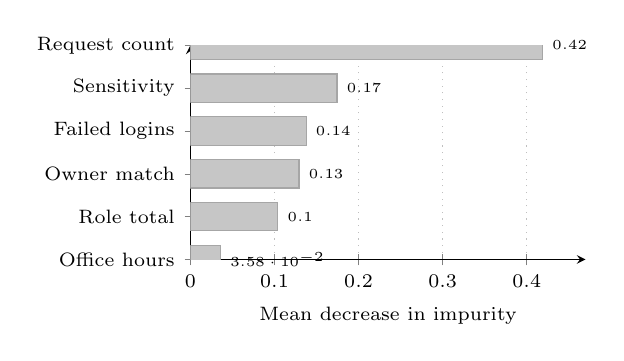
\begin{tikzpicture}
\begin{axis}[
  xbar, width=6.6cm, height=4.3cm,
  xmin=0, xmax=0.47,
  bar width=3.6mm,
  enlarge y limits=0.14,
  font=\scriptsize,
  xlabel={Mean decrease in impurity},
  symbolic y coords={Office hours,Role total,Owner match,Failed logins,Sensitivity,Request count},
  ytick=data,
  nodes near coords, nodes near coords style={font=\tiny},
  nodes near coords align=horizontal,
  axis lines=left,
  xmajorgrids, grid style={dotted,gray!50}
]
\addplot[fill=gray!45,draw=gray!70] coordinates {
 (0.0358,Office hours) (0.1040,Role total) (0.1292,Owner match)
 (0.1376,Failed logins) (0.1744,Sensitivity) (0.4189,Request count)};
\end{axis}
\end{tikzpicture}
\caption{Impurity-based feature importance of the trained forest; the three one-hot role
components are summed. Reported as a model diagnostic, not as causal evidence.}
\label{fig:importance}
\end{figure}

\subsection{Transpilation fidelity and inference cost}
\label{sec:parity}

The generated artifact is 2.9~MiB of plain JavaScript holding the 75 trees. We scored all 1{,}500
test rows through the JavaScript function and compared against the Python model: the predicted
label agreed on every row, and the largest absolute difference across all class probabilities was
$1.3\times10^{-15}$, i.e.\ floating-point noise. Compilation therefore costs nothing in accuracy.

Latency was measured inside Node.js with a high-resolution timer around each call, over 30{,}000
calls after warm-up; the reported values include timer overhead. Loading and parsing the module
takes 23.9~ms and the first call another 46.7~ms while the JIT compiles the tree cascades, both
once per process. Warm inference has a median of 23.6~$\mu$s, a mean of 25.7~$\mu$s, and stays
under 54.3~$\mu$s at the 99th percentile. This is roughly two orders of magnitude below the
1--2~ms that the two indexed audit queries cost, so the model is not the expensive part of the
added path; feature extraction is. Table~\ref{tab:runtime} collects these figures.

\begin{table}[t]
\caption{Transpiled artifact and measured per-request cost.}
\label{tab:runtime}
\centering
\footnotesize
\begin{tabular}{@{}ll@{}}
\toprule
Property & Value \\
\midrule
Artifact & 2.9~MiB JavaScript, 75 trees, no dependencies \\
Python--JS label agreement & 1500 / 1500 rows \\
Max probability deviation & $1.3\times10^{-15}$ \\
Module load + parse & 23.9~ms, once per process \\
First call (JIT) & 46.7~ms, once per process \\
Warm inference & 23.6~$\mu$s median, 37.9~$\mu$s p95, 54.3~$\mu$s p99 \\
Feature extraction & 1--2~ms (two indexed queries) \\
\bottomrule
\end{tabular}
\end{table}

\subsection{End-to-end exposure}

The integrated backend was exercised against records holding genuine AES-256-GCM ciphertext under
contexts engineered to land in each tier. Table~\ref{tab:exposure} reports what the same record
returns on each path. The \LOW{} path decrypts all seven fields. The \MED{} path performs exactly
two decryption calls, renders the account number as \texttt{****6789} from the stored last-four
column without touching its ciphertext, and withholds the four high-value identifiers. The
\HIGH{} path returns HTTP 403 with no decryption call executed at any point, which is the
behaviour required by~(\ref{eq:invariant}).

The practical effect is that one endpoint, one user and one record produce three different
responses depending only on runtime behaviour: full access up to roughly eight reads per minute,
masking between nine and thirteen, and refusal beyond about fifteen. Cross-record access to
sensitive data and a history of five or more failed logins move a request to refusal immediately,
irrespective of rate. A conventional pipeline with the same RBAC rules returns the full record in
every one of those cases.

\begin{table}[t]
\caption{Field-level exposure of the same encrypted record under the three policies.}
\label{tab:exposure}
\centering
\footnotesize
\begin{tabular}{@{}lccc@{}}
\toprule
Protected field & \LOW{} & \MED{} & \HIGH{} \\
\midrule
Branch name          & plain & plain & --- \\
Account holder name  & plain & masked initials & --- \\
Account number       & plain & \texttt{****6789}$^{*}$ & --- \\
Routing number       & plain & withheld & --- \\
SWIFT code           & plain & withheld & --- \\
IBAN                 & plain & withheld & --- \\
National identity no.& plain & withheld & --- \\
\midrule
Decryption calls     & 7 & 2 & \textbf{0} \\
Response             & 200 & 200 & 403 \\
\bottomrule
\end{tabular}

\smallskip
\parbox{\columnwidth}{\scriptsize $^{*}$Rendered from a separately stored plaintext last-four
column; the account-number ciphertext is never decrypted.}
\end{table}

\section{Discussion and Threats to Validity}

The most important limitation is the corpus. Training and testing both draw on a rule-generated
distribution, and a random forest represents rule conjunctions natively as root-to-leaf paths, so
part of the reported accuracy necessarily reflects the model recovering the labelling policy
rather than learning what abuse looks like in general. The 4\% noise floor, the overlapping
feature distributions and the sealed test partition prevent memorisation of individual rows, but
they cannot make the test partition come from a different generative process than the training
one. Repetition across five independent corpora shows the pipeline is stable, not that it
transfers. For this reason we state the 92.81\% refusal rate strictly under the defined synthetic
threat model, and we do not present it as evidence of real-world attack detection. The
architecture anticipates this: the audit tables accumulate genuine telemetry in exactly the
schema of the training features, which is the intended path to recalibration on production data.

Three narrower limitations should be noted. Per-request velocity features have a structural blind
spot for low-and-slow behaviour: an attacker who paces below the threshold is, in this feature
set, indistinguishable from a legitimate user, and no amount of training data changes that.
Closing it requires longer-horizon aggregates such as distinct records touched per hour or per
day. The behavioural counters live in
PostgreSQL, which is correct across application replicas but was not evaluated under
high-throughput multi-node load, where a distributed counter store would be the natural choice.
And the window sizes, the sensitivity tiers and the tier boundaries baked into the trained forest
were fixed by design rather than swept, so the framework currently requires retraining to change
a boundary --- calibrated probability thresholds would make that a configuration change instead.

A last point concerns what the classifier is allowed to affect. Its output can withhold data but
never grant more than static RBAC already permits, so a misclassification toward \HIGH{} is a
recoverable inconvenience while the layers beneath it remain in force. The reverse error is the
one that matters, and it is bounded by those same underlying controls rather than by the model.
Any deployment should be staged --- shadow scoring first, then masking, then refusal --- with
false-denial rates monitored across user segments and a human appeal path for contested denials.

\section{Conclusion}

We described a backend framework that treats decryption as the enforcement point rather than an
automatic consequence of retrieval. Protected fields survive ORM hydration as ciphertext, six
server-derived signals are scored in process by a transpiled random forest, and the predicted
risk tier decides whether a request receives the full record, a masked view, or a refusal issued
before any decryption call. On a quarantined synthetic partition the classifier reached 0.9780
accuracy and 0.9777 weighted F1, serving 99.14\% of legitimate requests in full while refusing
92.81\% of abusive ones, and the figures held at $0.9797 \pm 0.0033$ weighted F1 across five
independently generated corpora. The transpiled artifact reproduced the Python predictions
exactly on all 1{,}500 test rows and answered in 23.6~$\mu$s at the median, well below the cost
of the audit queries that feed it. End-to-end, the three paths performed 7, 2 and 0 field
decryptions.

What the results establish is that per-request exposure control is architecturally practical and
essentially free at runtime. What they do not establish is detection quality against real
attackers, which requires the operational telemetry the audit layer is designed to collect. That
substitution --- synthetic bootstrap replaced by production data, with calibrated thresholds and
longer-horizon features --- is the next step for this work.

\begin{thebibliography}{00}

\bibitem{gcm} M. Dworkin, ``Recommendation for block cipher modes of operation: Galois/Counter
Mode (GCM) and GMAC,'' NIST Special Publication 800-38D, Nov. 2007.

\bibitem{rbac} D. F. Ferraiolo, R. Sandhu, S. Gavrila, D. R. Kuhn, and R. Chandramouli,
``Proposed NIST standard for role-based access control,'' \emph{ACM Trans. Inf. Syst. Secur.},
vol. 4, no. 3, pp. 224--274, Aug. 2001.

\bibitem{abac} V. C. Hu \emph{et al.}, ``Guide to attribute based access control (ABAC)
definition and considerations,'' NIST Special Publication 800-162, updated Aug. 2019.

\bibitem{abacopen} D. Servos and S. L. Osborn, ``Current research and open problems in
attribute-based access control,'' \emph{ACM Comput. Surv.}, vol. 49, no. 4, pp. 1--45, 2017.

\bibitem{zta} S. Rose, O. Borchert, S. Mitchell, and S. Connelly, ``Zero trust architecture,''
NIST Special Publication 800-207, Aug. 2020.

\bibitem{zt5} K. A. Abuhasel, ``A zero-trust network-based access control scheme for sustainable
and resilient Industry 5.0,'' \emph{IEEE Access}, vol. 11, pp. 116398--116409, 2023.

\bibitem{rf} L. Breiman, ``Random forests,'' \emph{Machine Learning}, vol. 45, no. 1, pp. 5--32,
2001.

\bibitem{mlengine} A. Liu, X. Du, and N. Wang, ``Efficient access control permission decision
engine based on machine learning,'' \emph{Security and Communication Networks}, vol. 2021,
art. no. 3970485, 2021.

\bibitem{scada} M. Usman, M. S. Sarfraz, U. Habib, M. U. Aftab, and S. Javed, ``Automatic hybrid
access control in SCADA-enabled IIoT networks using machine learning,'' \emph{Sensors}, vol. 23,
no. 8, art. no. 3931, 2023.

\bibitem{survey} V. K. Matter, M. G. Martins, and J. L. V. Barbosa, ``Context-aware security and
machine learning for access control: A systematic mapping and taxonomies,'' \emph{Computer
Science Review}, vol. 60, art. no. 100880, 2025.

\bibitem{riskabac} R. Prajapati, S. S. Panchal, N. Soni, and S. R. Panchal, ``Machine
learning-based risk-adaptive attribute-based access control framework for secure IoT networks,''
\emph{Int. Res. J. Multidiscip. Technovation}, vol. 8, no. 3, pp. 495--519, 2026.

\bibitem{tde} V. Sidorov and W. K. Ng, ``Transparent data encryption for data-in-use and
data-at-rest in a cloud-based database-as-a-service solution,'' in \emph{Proc. IEEE World
Congress on Services}, 2015, pp. 221--228.

\bibitem{atrest} V. Shaik and K. Natarajan, ``Flexible and cost-effective cryptographic
encryption algorithm for securing unencrypted database files at rest and in transit,''
\emph{MethodsX}, vol. 9, art. no. 101924, 2022.

\bibitem{dbsurvey} E. F. Khalaf and M. M. Kadi, ``A survey of access control and data encryption
for database security,'' \emph{JKAU: Engineering Sciences}, vol. 28, no. 1, pp. 19--30, 2017.

\end{thebibliography}

\end{document}
